\documentclass[12pt,a4paper,oneside]{report}
\usepackage{fontspec}
\setmainfont{Latin Modern Roman}
\usepackage[margin=2.5cm]{geometry}
\usepackage{setspace}
\usepackage{amsmath}
\usepackage[unicode,hidelinks]{hyperref}
\onehalfspacing
\renewcommand{\contentsname}{Mục lục}
\renewcommand{\listfigurename}{Danh mục hình}
\renewcommand{\listtablename}{Danh mục bảng}
\renewcommand{\bibname}{Tài liệu tham khảo}
\renewcommand{\chaptername}{Chương}
\renewcommand{\figurename}{Hình}
\renewcommand{\tablename}{Bảng}
\begin{document}
\begin{titlepage}
\centering
{\Large [TÊN TRƯỜNG]\\[0.5cm] [TÊN KHOA/BỘ MÔN]\par}
\vspace{2cm}
{\Large BÀI TẬP LỚN MÔN TÍNH TOÁN SONG SONG\par}
\vspace{1cm}
{\LARGE\bfseries Parallel Breadth-First Search Using OpenMP:\\
Implementation, Optimization, and Performance Evaluation\par}
\vspace{1cm}
{\large Triển khai, tối ưu và đánh giá hiệu năng BFS song song\par}
\vspace{1.5cm}
Giảng viên hướng dẫn: [HỌ TÊN GIẢNG VIÊN]\\[0.6cm]
Nhóm sinh viên:\\
[THÀNH VIÊN 1 -- MSSV]\\
[THÀNH VIÊN 2 -- MSSV]\\
[THÀNH VIÊN 3 -- MSSV]
\vfill
[ĐỊA ĐIỂM], [THÁNG/NĂM]\\
\textbf{Bản khung bootstrap -- chưa có kết quả thực nghiệm}
\end{titlepage}
\pagenumbering{roman}
\chapter*{Tóm tắt}
\addcontentsline{toc}{chapter}{Tóm tắt}
Đề tài hướng tới xây dựng và đánh giá thuật toán tìm kiếm theo chiều rộng trên
CPU đa nhân bằng C11 và OpenMP. Bản hiện tại chỉ xác lập hợp đồng dữ liệu CSR,
giao diện thuật toán, quy trình kiểm thử và phương pháp đo thời gian.
Chưa triển khai BFS và chưa thu thập số liệu. Phần kết quả và kết luận về hiệu
năng sẽ được viết sau khi có thực nghiệm tái lập và kiểm chứng tính đúng đắn.
\tableofcontents
\clearpage
\listoffigures
\clearpage
\listoftables
\clearpage
\pagenumbering{arabic}
\chapter{Mở đầu}
\section{Bối cảnh và mục tiêu}
Tìm kiếm theo chiều rộng (BFS) là bài toán duyệt đồ thị theo khoảng cách tính
bằng số cạnh từ một đỉnh nguồn. Nhóm dự kiến triển khai một phiên bản tuần tự
và hai phiên bản OpenMP để nghiên cứu tính đúng đắn và chi phí song song hóa.
\section{Phạm vi}
Chương trình sử dụng C11, đồ thị CSR, OpenMP trên CPU và môi trường Windows.
Phiên bootstrap chỉ tạo hợp đồng và khung làm việc; chưa có thuật toán hoàn chỉnh.
\section{Nội dung cần bổ sung}
[BỔ SUNG: động cơ chọn đề tài, phân công ba thành viên và đóng góp thực tế sau triển khai.]

\chapter{Cơ sở lý thuyết}
\section{Đồ thị và BFS}
[BỔ SUNG: định nghĩa đồ thị có hướng/vô hướng, biểu diễn CSR, tính chất BFS,
chứng minh khoảng cách và độ phức tạp; bổ sung nguồn được kiểm chứng.]
\section{Hệ thống song song và OpenMP}
Giáo trình của Trobec và cộng sự là nguồn nền tảng dự kiến, tập trung vào Chương
2 về hệ thống song song và Chương 3 về OpenMP~\cite{trobec2018}.
[BỔ SUNG SAU KHI ĐỌC: shared memory, work sharing, atomic, barrier và scheduling.]
\section{Chỉ số hiệu năng}
Với thời gian tuần tự $T_s$ và thời gian song song $T_p$ trên $p$ luồng thực tế,
quy ước của thực nghiệm là $S_p=T_s/T_p$ và $E_p=S_p/p$.
Các thời gian đại diện sử dụng median theo quy trình thực nghiệm.

\chapter{Thiết kế và triển khai thuật toán BFS song song}
\section{Hợp đồng dữ liệu và API}
Đồ thị CSR là dữ liệu bất biến dùng chung. Số đỉnh được truyền tường minh để
giữ đỉnh cô lập. Distance có kiểu int32, nguồn bằng 0 và unreachable bằng $-1$.
Số cạnh báo cáo là số cung thực lưu trong CSR; cạnh vô hướng không phải self-loop
được lưu ở cả hai chiều. Hợp đồng chi tiết nằm trong docs/CONTRACT.md của mã nguồn.
\section{BFS tuần tự}
[CHƯA TRIỂN KHAI: thành viên phụ trách bổ sung thuật toán, giả mã và kiểm thử.]
\section{OpenMP cơ bản và tối ưu}
[CHƯA TRIỂN KHAI: mô tả claim visited, frontier, barrier giữa các mức;
giải thích an toàn bộ nhớ và lựa chọn static/dynamic/guided sau khi có code.]
\section{Nguồn tham khảo và giới hạn sử dụng}
Repository ParallelBFS được dùng làm nguồn khảo sát~\cite{parallelbfs}.
Bootstrap chưa audit thuật toán tại một commit cụ thể và không sao chép code
hoặc sử dụng số liệu README làm kết quả nhóm.

\chapter{Môi trường và phương pháp thực nghiệm}
\section{Thiết kế và điều kiện bắt đầu}
Thực nghiệm dự kiến so sánh Serial BFS, OpenMP Basic và OpenMP Optimized trên cùng đồ thị CSR, cùng nguồn và cùng quy tắc biểu diễn cạnh. Biến độc lập là phiên bản thuật toán, số luồng yêu cầu, chính sách lập lịch và cấu trúc/kích thước đồ thị. Đại lượng quan sát là tính đúng đắn, thời gian wall-clock, speedup, efficiency và độ biến thiên. Mỗi tổ hợp đồ thị, nguồn, thuật toán, số luồng và schedule là một cấu hình đo riêng; không gộp các nguồn thành các lần lặp của cùng một cấu hình.

Chỉ đo sau khi loader, serial và hai bản OpenMP đã merge, được review và vượt kiểm thử tính đúng đắn trên chính commit dùng để đo. CLI hiện gọi cả ba thuật toán thật và kiểm chứng đầu ra ngoài timer. Tuy nhiên chưa có phiên benchmark trên máy đo hợp lệ. Quy trình chi tiết và hợp đồng được quản lý tại \texttt{docs/EXPERIMENT\_PROTOCOL.md} và \texttt{docs/CONTRACT.md}. Chương này mô tả phương pháp dự kiến, chưa xác nhận thực nghiệm đã diễn ra.

\section{Môi trường và thông tin cần ghi nhận}
Khảo sát ngày 12/11/2026 xác nhận CPU Intel Core i5-12450HX (8 lõi vật lý, 12 luồng logic), Windows 11 Home Single Language phiên bản 10.0.26300, RAM hệ điều hành nhận 24\,866\,680 KiB và chế độ nguồn Balanced. Đây là máy dự kiến, chưa phải môi trường đã đo. GCC/UCRT64, Make, XeLaTeX và BibTeX không được tìm thấy trên PATH hoặc các vị trí chuẩn đã kiểm; Clang 14.0.6 có sẵn nhưng thiếu \texttt{omp.h}. Không cài phần mềm hoặc đổi chế độ nguồn. Bảng~\ref{tab:environment-plan} liệt kê metadata còn phải hoàn thiện khi máy đủ công cụ.
\begin{table}[htbp]
\centering\small
\caption{Metadata bắt buộc của phiên đo, bổ sung cho khảo sát máy.}
\label{tab:environment-plan}
\begin{tabular}{p{0.30\textwidth}p{0.58\textwidth}}
\toprule
Nhóm thông tin & Nội dung cần ghi \\
\midrule
Phần cứng & Model CPU; lõi vật lý/luồng logic; RAM \\
Phần mềm & Windows build; GCC và runtime; giá trị \texttt{\_OPENMP}; cờ biên dịch/liên kết \\
Điều kiện chạy & Nguồn điện; power mode; tải nền; affinity hoặc unset \\
Mã và cấu hình & Commit SHA, dirty state; lệnh; số luồng yêu cầu/thực tế; schedule \\
\bottomrule
\end{tabular}
\end{table}
Dự kiến thử $1,2,4,\ldots$ trong giới hạn số luồng logic đã xác minh, bổ sung mốc số lõi vật lý nếu khác. Không dùng quá số luồng logic cho phép so sánh chính. Tắt dynamic team bằng \texttt{OMP\_DYNAMIC=FALSE}; ghi giá trị thực của \texttt{OMP\_PROC\_BIND} và \texttt{OMP\_PLACES}, kể cả khi chưa đặt. Không giả định runtime hỗ trợ mọi chính sách affinity. Số luồng thực tế lấy từ \texttt{BFSMetrics} đo bên trong vùng xử lý BFS, không suy từ số luồng yêu cầu.

\section{Lựa chọn đồ thị và nguồn}
Tập tối thiểu gồm path, star và grid hai chiều, với vài kích thước tăng dần phù hợp bộ nhớ máy. Path tạo nhiều tầng hẹp, thích hợp khảo sát giới hạn song song theo tầng. Star có bậc rất không đều; nguồn ở tâm và ở lá tạo các mức công việc khác nhau, giúp kiểm tra ảnh hưởng của vị trí nguồn. Grid có cấu trúc đều hơn và frontier thay đổi dần theo tầng, cung cấp đối chứng cho hai trường hợp trên. Đồ thị ngẫu nhiên với seed cố định có thể bổ sung để khảo sát phân bố bậc khác; chỉ thêm dữ liệu công khai khi đã kiểm tra giấy phép, nguồn tải và dung lượng. Đây là lựa chọn thiết kế, chưa có dataset đã được chốt.

Đồ thị nhỏ dùng kiểm chứng bằng tay; đồ thị lớn hơn dùng đánh giá thời gian. Dữ liệu tự sinh phục vụ thực nghiệm phải ghi rõ tự sinh, thuật toán sinh và tham số; thời gian thu được vẫn phải do chương trình thực chạy. Không sử dụng dữ liệu thời gian giả. Kích thước cụ thể được chốt sau kiểm tra tài nguyên, trước khi xem kết quả so sánh. Danh sách nguồn được cố định trước đo: ít nhất một nguồn cho mỗi đồ thị và nguồn bổ sung có chủ đích để kiểm tra độ nhạy; không chỉ chọn nguồn đem lại speedup tốt.

Mỗi dataset cần URL hoặc lệnh sinh, giấy phép nếu có, SHA-256, seed, số đỉnh, số dòng cạnh đầu vào và số cung CSR, hướng cạnh, nguồn và số đỉnh tới được. Số đỉnh phải tường minh để giữ isolates. Với vô hướng, cạnh không phải self-loop được lưu hai chiều; self-loop lưu một cung, cạnh trùng được giữ. Vì vậy số dòng đầu vào không được dùng thay số cung CSR khi so sánh khối lượng công việc.

\section{Kiểm chứng tính đúng đắn}
Serial trước hết phải khớp khoảng cách tính tay trên đồ thị nhỏ; không mặc định serial là oracle đúng. Bộ trường hợp gồm một đỉnh, không cạnh, path, star, diamond, chu trình, đồ thị rời rạc/đỉnh cô lập, self-loop và cạnh trùng, cả có hướng/vô hướng và nhiều nguồn. Sau đó so mọi phần tử distance của từng bản OpenMP với serial đã xác minh, gồm nguồn bằng 0 và unreachable bằng $-1$. Số đỉnh tới được bằng nhau chưa đủ chứng minh mảng khoảng cách bằng nhau.

Lặp kiểm thử qua số luồng và static/dynamic/guided để phát hiện lỗi không ổn định; đồng thời review atomic claim, công bố distance, barrier giữa tầng và dung lượng frontier. Test lặp thành công không chứng minh tuyệt đối không có race. Kiểm tra input lỗi, overflow, ownership và việc CSR không bị sửa là các kiểm thử riêng. Khi lỗi trạng thái, metrics không hợp lệ hoặc distance sai, giữ log và không nhận thời gian đó vào thống kê thành công. Validation được thực hiện ngoài khoảng đo, không làm thay đổi đầu ra trước khi đối chiếu.

\section{Đo thời gian và tổ chức lần chạy}
Dùng \texttt{omp\_get\_wtime()} ngay trước và sau một lời gọi BFS trên cùng luồng gọi. Hàm trả wall-clock theo giây; đặc tả không bảo đảm đồng hồ nhất quán giữa các luồng~\cite{openmpwtime}. Đặt $t_i=t_{\mathrm{end}}-t_{\mathrm{start}}$. Khoảng đo bao gồm khởi tạo distance, cấp phát/giải phóng scratch và đồng bộ nằm trong BFS; loại đọc file, dựng CSR, cấp phát output của caller, kiểm chứng và ghi kết quả. Không trừ overhead ước lượng khỏi mẫu đo.

Mỗi cấu hình có một warm-up không đưa vào thống kê và ít nhất 10 mẫu đo. Đảo thứ tự cấu hình bằng seed cố định, lưu thứ tự thực tế để giảm sai lệch do nhiệt và tải nền. Dùng cùng chính sách warm-up cho mọi thuật toán; không gọi đây là phép đo cold-cache. Nếu mẫu quá ngắn so với độ phân giải đồng hồ hoặc overhead, ghi hạn chế và chọn thêm kích thước lớn hơn, không gán thời gian bằng một giá trị tùy ý.

Mỗi mẫu thành công lưu JSONL schema v1; serial ghi schedule là \texttt{none}, số luồng thực tế là 1. Mẫu lỗi, stderr, warm-up và thứ tự chạy vẫn được lưu. Mỗi phiên dùng thư mục mới, không ghi đè raw. Manifest liên kết SHA mã, lệnh, metadata môi trường/dataset, trạng thái kiểm chứng, chỉ số lần lặp và SHA-256 các tệp. Chỉ sinh bảng/biểu đồ từ raw đã đối chiếu manifest, bằng lệnh có thể chạy lại.

\section{Thống kê và chỉ số hiệu năng}
Với mỗi cấu hình hợp lệ, báo số mẫu, median, min, max và khoảng tứ phân vị $IQR=Q_3-Q_1$. Quy ước tính phân vị dự kiến là nội suy tuyến tính tại chỉ số $(N-1)q$ trên dãy tăng dần (đánh số từ 0); script phân tích hiện giữ quy ước này. Không âm thầm bỏ outlier; lỗi hoặc lần chạy bị gián đoạn được ghi riêng cùng lý do. IQR mô tả độ phân tán, không được trình bày như khoảng tin cậy.

Gọi $\widetilde T_s$ là median serial và $\widetilde T_{a,p}$ là median bản OpenMP $a$ có team thực tế ổn định $p$ trên cùng đồ thị, nguồn và build:
\[
S_{a,p}=\frac{\widetilde T_s}{\widetilde T_{a,p}},\qquad
E_{a,p}=\frac{S_{a,p}}{p}.
\]
Efficiency có thể biểu diễn phần trăm bằng $100E_{a,p}$. Đây là tỉ số các median, không phải median các tỉ số ghép cặp. Nếu median bằng 0 hoặc team thay đổi, đánh dấu không so sánh hoặc tách nhóm đủ mẫu; không chia cho 0 hay lấy số luồng yêu cầu thay thế. Scaling so với OpenMP một luồng là $\widetilde T_{a,1}/\widetilde T_{a,p}$, một đại lượng riêng không thay speedup so serial.

\section{Tính công bằng và giới hạn}
Giữ cùng CSR semantics, dataset, nguồn, compiler, flags tối ưu và ranh giới timer. Khảo sát static/dynamic/guided trên cùng ma trận cấu hình; không chọn schedule tốt nhất sau đo mà bỏ các trường hợp chậm. Đo tuần tự từng cấu hình, hạn chế tải nền và giữ điều kiện nguồn điện ổn định. Nếu điều kiện thay đổi đáng kể, tách phiên và ghi nhận thay vì gộp vô điều kiện.

Kết quả trên một máy và số ít cấu trúc không đại diện mọi CPU hoặc đồ thị. SMT, cache, băng thông bộ nhớ, nhiệt và tải nền có thể ảnh hưởng thời gian. Nhiều lần lặp trong một phiên không thay cho tái lập trên máy khác. Timer tổng không đủ tách định lượng thời gian barrier, contention hay cache miss; các giải thích này chỉ là giả thuyết phù hợp thiết kế nếu chưa có đo bổ sung. Tên bản tối ưu không bảo đảm tăng tốc; slowdown cũng là kết quả cần trình bày trung thực.

\chapter{Kết quả thực nghiệm và đánh giá}
\section{Tính toàn vẹn dữ liệu và kết quả tổng quát}
Thực nghiệm chính thức ngày 12/11/2026 bắt đầu lúc 16:32:58 và kết thúc lúc 16:42:26 (UTC+7), khoảng 9 phút 28 giây, trên commit \texttt{ab588fb}. Chín phiên đều có đúng 275 lượt: 25 warm-up và 250 mẫu chính thức; tổng 2250 mẫu được nhận, không lỗi, timeout hoặc mẫu bị loại. Requested và actual threads khớp tại 1/2/4/8. Analyzer kiểm hash, đầy đủ cấu hình, warm-up và chỉ số lần lặp trước khi tổng hợp. Bản sao ổ D được đối chiếu từng file.

Giám sát ghi nguồn AC trong toàn bộ phiên; RAM trống thấp nhất 11\,135\,807\,488 byte (khoảng 10,37 GiB). Tải CPU nền đo một giây trước mỗi phiên nằm trong khoảng 1,30--19,01\%; đây không phải tải nền đo liên tục trong BFS. Không có số đo nhiệt độ để khẳng định máy không throttling. Toàn bộ bảng/biểu đồ dùng raw thật, không dùng timing CI hoặc fixture unit test.

\textbf{Không có cấu hình OpenMP nào nhanh hơn Serial trên ma trận này.} Trong 216 cấu hình OpenMP, speedup lớn nhất là 0,2914 ở Optimized một luồng/static/grid512 nguồn 0 (5,814 ms so Serial 1,6942 ms). Khi xét team từ hai luồng, scaling so OpenMP một luồng lớn nhất cũng chỉ 0,7536 ở Basic hai luồng/static/star một triệu đỉnh. Đây là kết quả của phép đo lời gọi độc lập trên tập dữ liệu đã chốt, không phải kết luận mọi BFS song song đều chậm.

\begin{table}[htbp]\centering\small
\caption{Ba đồ thị lớn, nguồn 0, static, actual 8; median theo ms, speedup so Serial, 10 mẫu/cấu hình.}\label{tab:headline}
\begin{tabular}{lrrrrr}\toprule
Đồ thị & Serial & Basic8 & Opt8 & $S_{B,8}$ & $S_{O,8}$ \\\midrule
Path8192 & 0,05185 & 922,0907 & 1562,0243 & 0,00005623 & 0,00003319 \\
Star1000000 & 3,1294 & 26,4158 & 26,4872 & 0,1185 & 0,1181 \\
Grid512 & 1,6942 & 112,6744 & 179,7294 & 0,01504 & 0,009426 \\\bottomrule
\end{tabular}\end{table}

\section{Bảng thống kê theo cấu hình}
Các bảng sau trình bày mọi mức luồng với static: Serial baseline, median, IQR, speedup, efficiency theo team thực và scaling so OpenMP một luồng. Không chọn schedule thắng để thay ma trận. Tệp đi kèm \texttt{results/experiment-20261112/summary.csv} chứa đầy đủ 225 dòng với cả static/dynamic/guided, min, max, $Q_1$ và $Q_3$. Serial là một baseline cho mỗi đồ thị/nguồn. Số hiển thị được làm tròn; phép tính và tệp máy đọc giữ độ chính xác gốc.
\begin{table}[htbp]
\centering\small
\caption[path2048-s0: thống kê static]{path2048-s0: median và IQR theo ms, static; 10 mẫu/cấu hình. $S$ so Serial, $E$ theo team thực, $C$ so OpenMP một luồng.}
\label{tab:path2048-s0}
\begin{tabular}{lrrrrrr}
\toprule
Phiên bản & $p$ & Median & IQR & $S$ & $E$ (\%) & $C$ \\
\midrule
Serial & 1 & 0,0097 & 0 & 1 & 100 & -- \\
Basic & 1 & 0,2198 & 0,0123 & 0,04414 & 4,414 & 1 \\
Basic & 2 & 59,01 & 2,527 & 0,0001644 & 0,008219 & 0,003724 \\
Basic & 4 & 123,4 & 3,985 & $7,858\times10^{-5}$ & 0,001965 & 0,00178 \\
Basic & 8 & 229,4 & 16,84 & $4,228\times10^{-5}$ & 0,0005284 & 0,0009577 \\
Optimized & 1 & 0,2786 & 0,005475 & 0,03481 & 3,481 & 1 \\
Optimized & 2 & 97,08 & 2,486 & $9,991\times10^{-5}$ & 0,004996 & 0,00287 \\
Optimized & 4 & 204,8 & 5,98 & $4,737\times10^{-5}$ & 0,001184 & 0,001361 \\
Optimized & 8 & 390 & 20,15 & $2,487\times10^{-5}$ & 0,0003109 & 0,0007146 \\
\bottomrule
\end{tabular}
\end{table}

\begin{table}[htbp]
\centering\small
\caption[path8192-s0: thống kê static]{path8192-s0: median và IQR theo ms, static; 10 mẫu/cấu hình. $S$ so Serial, $E$ theo team thực, $C$ so OpenMP một luồng.}
\label{tab:path8192-s0}
\begin{tabular}{lrrrrrr}
\toprule
Phiên bản & $p$ & Median & IQR & $S$ & $E$ (\%) & $C$ \\
\midrule
Serial & 1 & 0,05185 & 0,006975 & 1 & 100 & -- \\
Basic & 1 & 0,6653 & 0,01063 & 0,07793 & 7,793 & 1 \\
Basic & 2 & 238,1 & 10,31 & 0,0002178 & 0,01089 & 0,002794 \\
Basic & 4 & 493,6 & 15,19 & 0,0001051 & 0,002626 & 0,001348 \\
Basic & 8 & 922,1 & 45,46 & $5,623\times10^{-5}$ & 0,0007029 & 0,0007215 \\
Optimized & 1 & 0,8969 & 0,01422 & 0,05781 & 5,781 & 1 \\
Optimized & 2 & 392 & 4,749 & 0,0001323 & 0,006613 & 0,002288 \\
Optimized & 4 & 831,2 & 16,72 & $6,238\times10^{-5}$ & 0,001559 & 0,001079 \\
Optimized & 8 & 1562 & 76,62 & $3,319\times10^{-5}$ & 0,0004149 & 0,0005742 \\
\bottomrule
\end{tabular}
\end{table}

\begin{table}[htbp]
\centering\small
\caption[path8192-s4096: thống kê static]{path8192-s4096: median và IQR theo ms, static; 10 mẫu/cấu hình. $S$ so Serial, $E$ theo team thực, $C$ so OpenMP một luồng.}
\label{tab:path8192-s4096}
\begin{tabular}{lrrrrrr}
\toprule
Phiên bản & $p$ & Median & IQR & $S$ & $E$ (\%) & $C$ \\
\midrule
Serial & 1 & 0,0372 & 0,0034 & 1 & 100 & -- \\
Basic & 1 & 0,4464 & 0,0103 & 0,08332 & 8,332 & 1 \\
Basic & 2 & 116,8 & 4,529 & 0,0003186 & 0,01593 & 0,003824 \\
Basic & 4 & 243,1 & 6,511 & 0,0001531 & 0,003826 & 0,001837 \\
Basic & 8 & 468,4 & 18,49 & $7,941\times10^{-5}$ & 0,0009926 & 0,000953 \\
Optimized & 1 & 0,5499 & 0,008075 & 0,06765 & 6,765 & 1 \\
Optimized & 2 & 194,3 & 3,152 & 0,0001915 & 0,009575 & 0,002831 \\
Optimized & 4 & 409,8 & 14,78 & $9,078\times10^{-5}$ & 0,00227 & 0,001342 \\
Optimized & 8 & 767 & 42,57 & $4,85\times10^{-5}$ & 0,0006062 & 0,0007169 \\
\bottomrule
\end{tabular}
\end{table}

\begin{table}[htbp]
\centering\small
\caption[star100000-s0: thống kê static]{star100000-s0: median và IQR theo ms, static; 10 mẫu/cấu hình. $S$ so Serial, $E$ theo team thực, $C$ so OpenMP một luồng.}
\label{tab:star100000-s0}
\begin{tabular}{lrrrrrr}
\toprule
Phiên bản & $p$ & Median & IQR & $S$ & $E$ (\%) & $C$ \\
\midrule
Serial & 1 & 0,2825 & 0,1892 & 1 & 100 & -- \\
Basic & 1 & 1,811 & 0,1583 & 0,156 & 15,6 & 1 \\
Basic & 2 & 3,459 & 0,5684 & 0,08167 & 4,084 & 0,5236 \\
Basic & 4 & 3,872 & 1,072 & 0,07296 & 1,824 & 0,4678 \\
Basic & 8 & 4,332 & 0,9949 & 0,06521 & 0,8151 & 0,4181 \\
Optimized & 1 & 1,529 & 0,1227 & 0,1848 & 18,48 & 1 \\
Optimized & 2 & 3,089 & 0,4858 & 0,09145 & 4,572 & 0,4949 \\
Optimized & 4 & 3,681 & 0,5019 & 0,07675 & 1,919 & 0,4154 \\
Optimized & 8 & 4,386 & 0,3927 & 0,06441 & 0,8051 & 0,3486 \\
\bottomrule
\end{tabular}
\end{table}

\begin{table}[htbp]
\centering\small
\caption[star1000000-s0: thống kê static]{star1000000-s0: median và IQR theo ms, static; 10 mẫu/cấu hình. $S$ so Serial, $E$ theo team thực, $C$ so OpenMP một luồng.}
\label{tab:star1000000-s0}
\begin{tabular}{lrrrrrr}
\toprule
Phiên bản & $p$ & Median & IQR & $S$ & $E$ (\%) & $C$ \\
\midrule
Serial & 1 & 3,129 & 0,1779 & 1 & 100 & -- \\
Basic & 1 & 17,68 & 0,7979 & 0,177 & 17,7 & 1 \\
Basic & 2 & 23,46 & 1,176 & 0,1334 & 6,67 & 0,7536 \\
Basic & 4 & 25,23 & 1,81 & 0,124 & 3,101 & 0,7007 \\
Basic & 8 & 26,42 & 1,165 & 0,1185 & 1,481 & 0,6693 \\
Optimized & 1 & 15,44 & 0,6806 & 0,2027 & 20,27 & 1 \\
Optimized & 2 & 23,23 & 1,789 & 0,1347 & 6,735 & 0,6645 \\
Optimized & 4 & 23,03 & 1,533 & 0,1359 & 3,397 & 0,6702 \\
Optimized & 8 & 26,49 & 2,311 & 0,1181 & 1,477 & 0,5828 \\
\bottomrule
\end{tabular}
\end{table}

\begin{table}[htbp]
\centering\small
\caption[star1000000-s1: thống kê static]{star1000000-s1: median và IQR theo ms, static; 10 mẫu/cấu hình. $S$ so Serial, $E$ theo team thực, $C$ so OpenMP một luồng.}
\label{tab:star1000000-s1}
\begin{tabular}{lrrrrrr}
\toprule
Phiên bản & $p$ & Median & IQR & $S$ & $E$ (\%) & $C$ \\
\midrule
Serial & 1 & 3,189 & 0,4142 & 1 & 100 & -- \\
Basic & 1 & 17,08 & 0,3277 & 0,1867 & 18,67 & 1 \\
Basic & 2 & 23,34 & 1,094 & 0,1367 & 6,833 & 0,7319 \\
Basic & 4 & 23,91 & 1,421 & 0,1334 & 3,334 & 0,7142 \\
Basic & 8 & 26,27 & 1,562 & 0,1214 & 1,517 & 0,6501 \\
Optimized & 1 & 15,51 & 0,9614 & 0,2056 & 20,56 & 1 \\
Optimized & 2 & 24,04 & 2,199 & 0,1326 & 6,632 & 0,645 \\
Optimized & 4 & 23,76 & 0,859 & 0,1342 & 3,355 & 0,6526 \\
Optimized & 8 & 25,63 & 1,863 & 0,1244 & 1,555 & 0,605 \\
\bottomrule
\end{tabular}
\end{table}

\begin{table}[htbp]
\centering\small
\caption[grid128-s0: thống kê static]{grid128-s0: median và IQR theo ms, static; 10 mẫu/cấu hình. $S$ so Serial, $E$ theo team thực, $C$ so OpenMP một luồng.}
\label{tab:grid128-s0}
\begin{tabular}{lrrrrrr}
\toprule
Phiên bản & $p$ & Median & IQR & $S$ & $E$ (\%) & $C$ \\
\midrule
Serial & 1 & 0,0912 & 0,0241 & 1 & 100 & -- \\
Basic & 1 & 0,5634 & 0,02492 & 0,1619 & 16,19 & 1 \\
Basic & 2 & 8,678 & 0,4216 & 0,01051 & 0,5255 & 0,06492 \\
Basic & 4 & 16,01 & 0,7455 & 0,005697 & 0,1424 & 0,03519 \\
Basic & 8 & 30,53 & 2,488 & 0,002987 & 0,03734 & 0,01846 \\
Optimized & 1 & 0,4789 & 0,01635 & 0,1904 & 19,04 & 1 \\
Optimized & 2 & 13,25 & 0,1796 & 0,006884 & 0,3442 & 0,03615 \\
Optimized & 4 & 26,43 & 0,8346 & 0,003451 & 0,08627 & 0,01812 \\
Optimized & 8 & 49,01 & 4,316 & 0,001861 & 0,02326 & 0,009773 \\
\bottomrule
\end{tabular}
\end{table}

\begin{table}[htbp]
\centering\small
\caption[grid512-s0: thống kê static]{grid512-s0: median và IQR theo ms, static; 10 mẫu/cấu hình. $S$ so Serial, $E$ theo team thực, $C$ so OpenMP một luồng.}
\label{tab:grid512-s0}
\begin{tabular}{lrrrrrr}
\toprule
Phiên bản & $p$ & Median & IQR & $S$ & $E$ (\%) & $C$ \\
\midrule
Serial & 1 & 1,694 & 0,3032 & 1 & 100 & -- \\
Basic & 1 & 7,043 & 0,5137 & 0,2405 & 24,05 & 1 \\
Basic & 2 & 37,73 & 2,058 & 0,04491 & 2,245 & 0,1867 \\
Basic & 4 & 63,98 & 3,206 & 0,02648 & 0,662 & 0,1101 \\
Basic & 8 & 112,7 & 8,654 & 0,01504 & 0,188 & 0,06251 \\
Optimized & 1 & 5,814 & 0,5139 & 0,2914 & 29,14 & 1 \\
Optimized & 2 & 52,54 & 4,019 & 0,03224 & 1,612 & 0,1106 \\
Optimized & 4 & 92,22 & 3,916 & 0,01837 & 0,4593 & 0,06305 \\
Optimized & 8 & 179,7 & 3,178 & 0,009426 & 0,1178 & 0,03235 \\
\bottomrule
\end{tabular}
\end{table}

\begin{table}[htbp]
\centering\small
\caption[grid512-s131328: thống kê static]{grid512-s131328: median và IQR theo ms, static; 10 mẫu/cấu hình. $S$ so Serial, $E$ theo team thực, $C$ so OpenMP một luồng.}
\label{tab:grid512-s131328}
\begin{tabular}{lrrrrrr}
\toprule
Phiên bản & $p$ & Median & IQR & $S$ & $E$ (\%) & $C$ \\
\midrule
Serial & 1 & 1,871 & 0,2011 & 1 & 100 & -- \\
Basic & 1 & 7,302 & 0,1272 & 0,2563 & 25,63 & 1 \\
Basic & 2 & 27,8 & 1,454 & 0,0673 & 3,365 & 0,2626 \\
Basic & 4 & 39,91 & 1,358 & 0,04688 & 1,172 & 0,1829 \\
Basic & 8 & 62,39 & 2,516 & 0,02999 & 0,3749 & 0,117 \\
Optimized & 1 & 6,68 & 0,6215 & 0,2801 & 28,01 & 1 \\
Optimized & 2 & 30,81 & 2,338 & 0,06072 & 3,036 & 0,2168 \\
Optimized & 4 & 52,66 & 1,867 & 0,03553 & 0,8883 & 0,1269 \\
Optimized & 8 & 92,55 & 2,286 & 0,02022 & 0,2527 & 0,07218 \\
\bottomrule
\end{tabular}
\end{table}

\clearpage

\section{Path: giới hạn của frontier hẹp}
Với nguồn 0, tăng path từ 2048 lên 8192 đỉnh (gấp4) làm median Serial tăng từ 0,0097 lên 0,05185 ms; Basic8/static từ 229,45 lên 922,09 ms, gần gấp4. Optimized 8/static từ 389,96 lên 1562,02 ms. Frontier chỉ có một đỉnh mỗi mức, nên tăng team không cung cấp thêm đỉnh cùng tầng để chia. Chi phí đồng bộ theo hàng nghìn mức phù hợp với xu hướng này; timer tổng chưa định lượng riêng barrier.

Basic một luồng/static mất0,6653 ms ở path8192, khoảng 12,8 lần Serial; actual 8 mất922,09 ms. Optimized 8 chậm hơn Basic8 khoảng 1,694 lần. Không thể giải thích toàn bộ chênh lệch chỉ bằng khởi tạo team một lần: tổ chức frontier/visited, lịch trình và đồng bộ lặp theo mức cũng có thể góp phần, cần profiling để tách riêng.

Đổi nguồn từ 0 sang 4096 giảm khoảng cách lớn nhất từ 8191 xuống4096. Basic8/static còn 468,45 ms (giảm 49,2\%), Optimized còn 767,02 ms (giảm 50,9\%). Quan sát phù hợp số mức giảm, nhưng hai nguồn chạy ở phiên riêng nên còn sai lệch thời điểm/tải nền. Cả hai vẫn chậm hơn Serial. Hình~\ref{fig:path-runtime}--\ref{fig:path-schedule} trình bày toàn bộ schedule và team.

\begin{figure}[p]\centering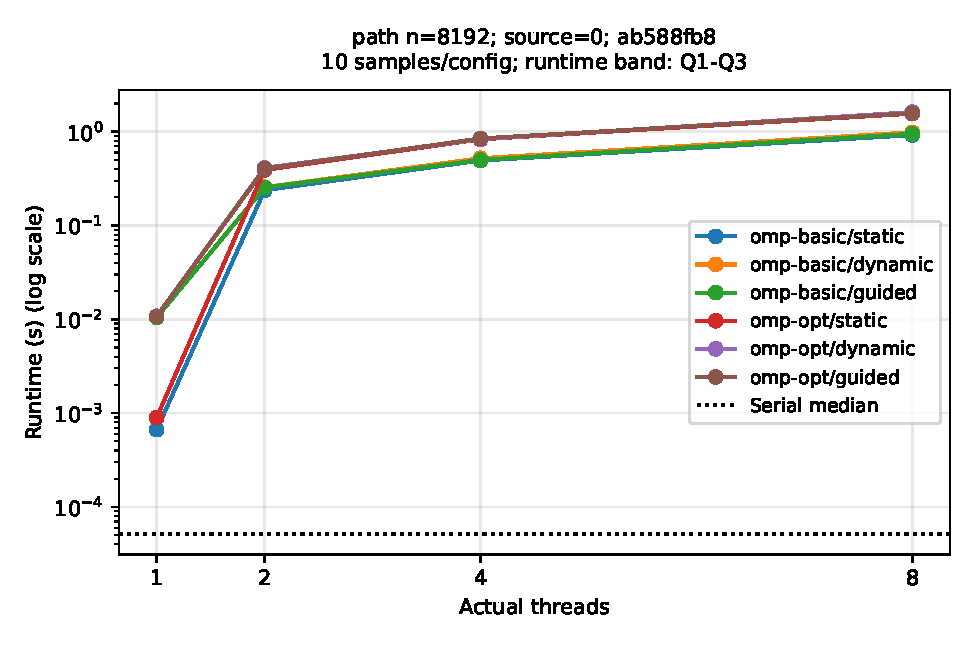
\includegraphics[width=.94\textwidth]{figures/experiment-20261112/path8192-s0/median.pdf}
\caption[Path8192: thời gian]{Path8192, nguồn 0, ab588fb: median và dải $Q_1$--$Q_3$, 10 mẫu/cấu hình; trục thời gian log để thấy cả Serial.}\label{fig:path-runtime}\end{figure}
\begin{figure}[p]\centering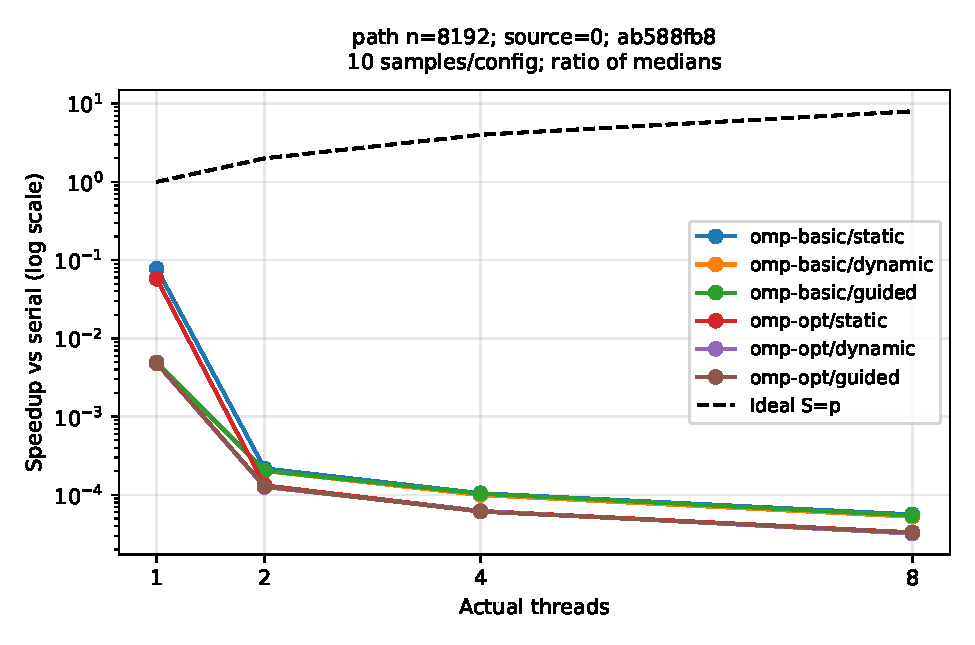
\includegraphics[width=.94\textwidth]{figures/experiment-20261112/path8192-s0/speedup.pdf}
\caption[Path8192: speedup]{Path8192, nguồn 0: speedup so Serial trên trục log; $S=p$ là mốc lý tưởng, không phải số đo.}\label{fig:path-speedup}\end{figure}
\begin{figure}[p]\centering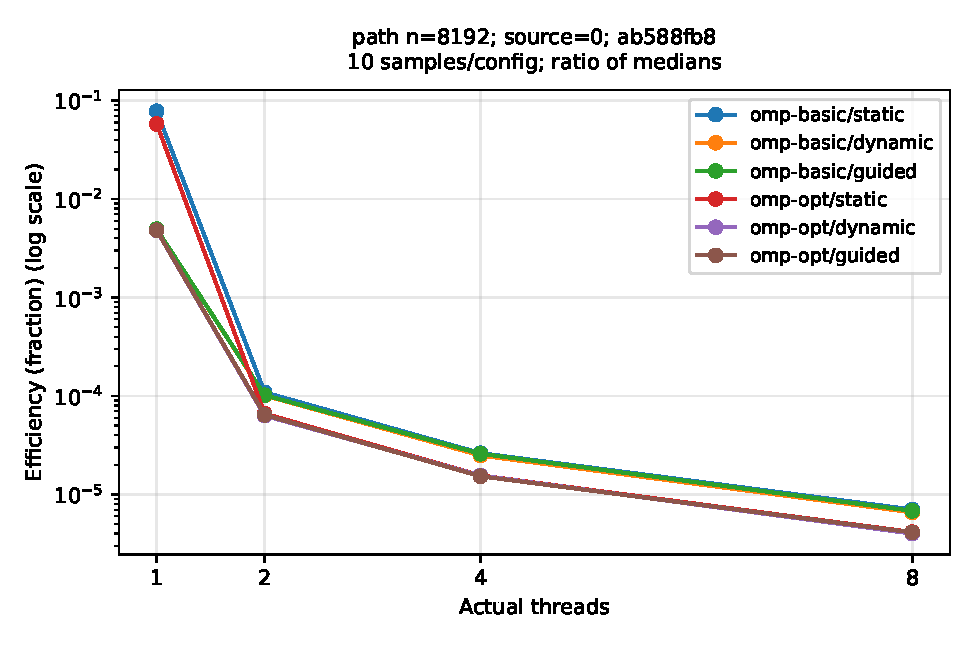
\includegraphics[width=.94\textwidth]{figures/experiment-20261112/path8192-s0/efficiency.pdf}
\caption[Path8192: efficiency]{Path8192, nguồn 0: efficiency $S/p$ theo team thực, 10 mẫu/cấu hình, commit ab588fb.}\label{fig:path-efficiency}\end{figure}
\begin{figure}[p]\centering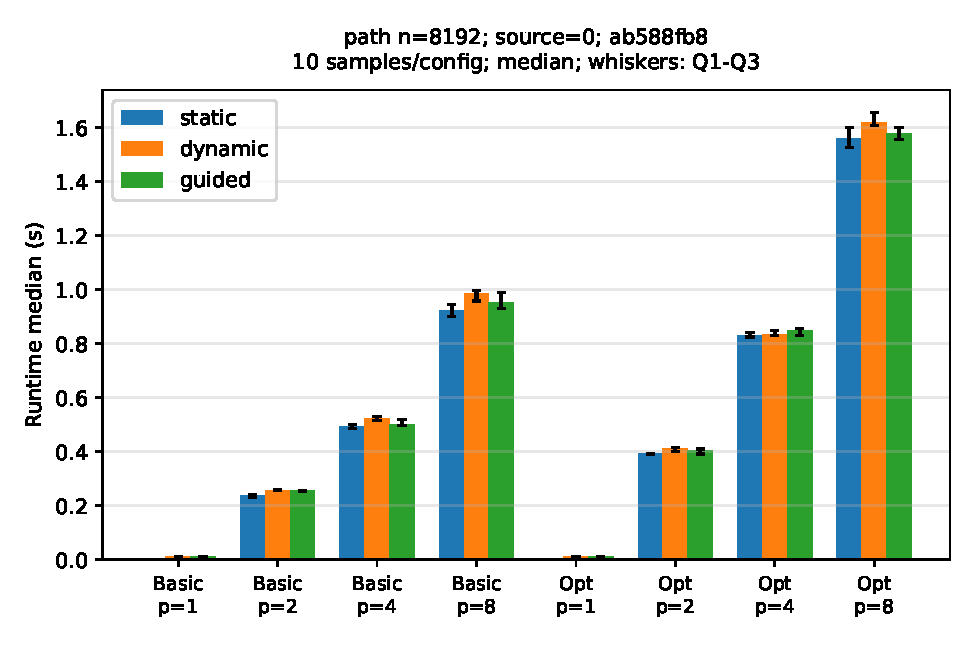
\includegraphics[width=.94\textwidth]{figures/experiment-20261112/path8192-s0/scheduling.pdf}
\caption[Path8192: scheduling]{Path8192, nguồn 0: scheduling trong cùng thuật toán/team; cột là median, thanh sai số là $Q_1$--$Q_3$.}\label{fig:path-schedule}\end{figure}
\clearpage

\section{Star: bậc lệch và chi phí lập lịch}
Star một triệu đỉnh có Serial median 3,1294 ms. Static/actual 8 cho Basic26,4158 ms và Optimized 26,4872 ms; speedup khoảng 0,118, efficiency khoảng 1,48\%. Hai median chênh0,0714 ms, nhỏ hơn IQR của mỗi bản (1,1649 và 2,3114 ms); chưa đủ cơ sở gọi Optimized tốt hơn. Ở bốn luồng/static, Optimized 23,0336 ms thấp hơn Basic25,2312 ms khoảng 8,7\%, nhưng lợi ích không nhất quán qua số luồng và vẫn chậm hơn Serial.

Đỉnh tâm có bậc999999 nhưng chỉ do một lần lặp frontier xử lý; vòng láng giềng trong một đỉnh không được chia cho nhiều luồng. Frontier sau đó rộng nhưng mỗi lá chỉ có một cung về tâm đã thăm. Nhiều đỉnh không đồng nghĩa nhiều công việc hữu ích cân bằng ở mọi mức; bỏ bộ đếm frontier chung chưa đủ bảo đảm tăng tốc.

Ở actual 8, dynamic làm Basic tăng từ 26,4158 lên 98,8135 ms (3,74 lần), Optimized từ 26,4872 lên 101,2997 ms (3,82 lần). Guided là 27,2610 và 26,1920 ms, gần static hơn. Điều này phù hợp giả thuyết chi phí cấp phát nhiều đơn vị việc nhỏ khi quét các lá; chưa phải đo riêng bộ lập lịch.

Nguồn lá1 cho Basic8/static 26,2714 ms và Optimized 25,6343 ms, chỉ khác khoảng 0,5--3,2\% so nguồn tâm trong khi IQR cỡ1,6--1,9 ms. Không kết luận lợi ích nguồn lá ổn định. Tăng kích thước từ 100000 lên 1000000 làm Serial median tăng11,1 lần, Basic8/static tăng6,1 lần, nhưng chưa tạo $S>1$. Xem Hình~\ref{fig:star-runtime}--\ref{fig:star-schedule}.

\begin{figure}[p]\centering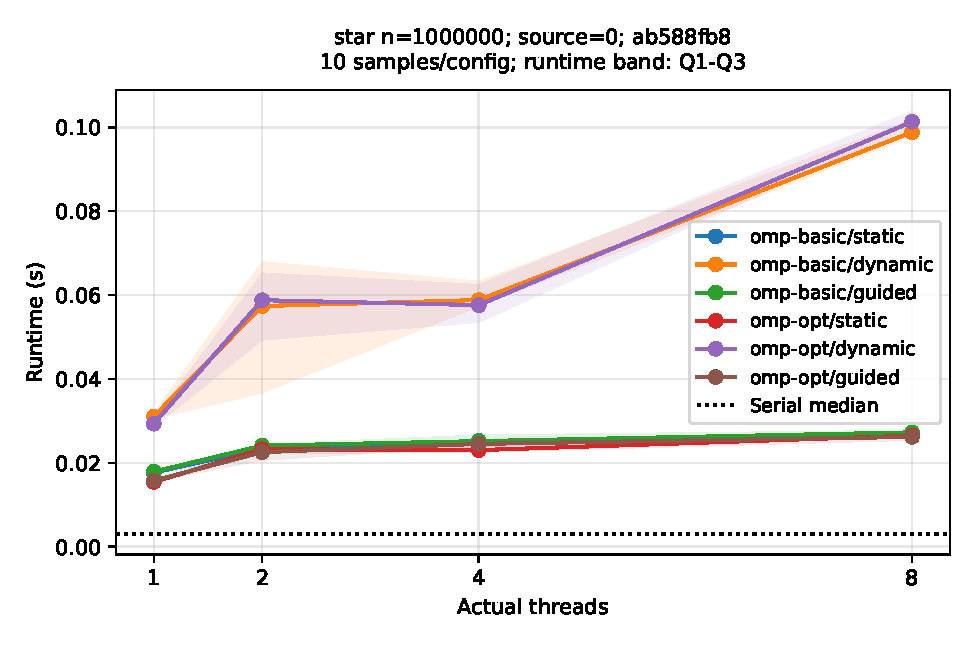
\includegraphics[width=.94\textwidth]{figures/experiment-20261112/star1000000-s0/median.pdf}
\caption[Star1000000: thời gian]{Star1000000, nguồn 0: median và dải IQR thời gian, 10 mẫu/cấu hình, commit ab588fb.}\label{fig:star-runtime}\end{figure}
\begin{figure}[p]\centering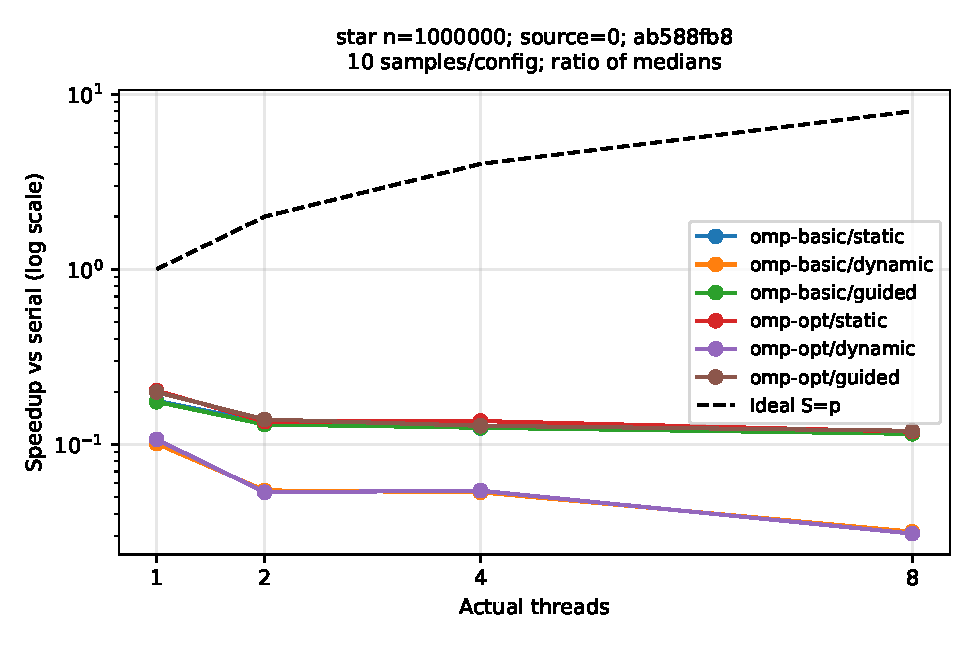
\includegraphics[width=.94\textwidth]{figures/experiment-20261112/star1000000-s0/speedup.pdf}
\caption[Star1000000: speedup]{Star1000000, nguồn 0: speedup so Serial và mốc $S=p$ trên trục log; mọi cấu hình dưới 1.}\label{fig:star-speedup}\end{figure}
\begin{figure}[p]\centering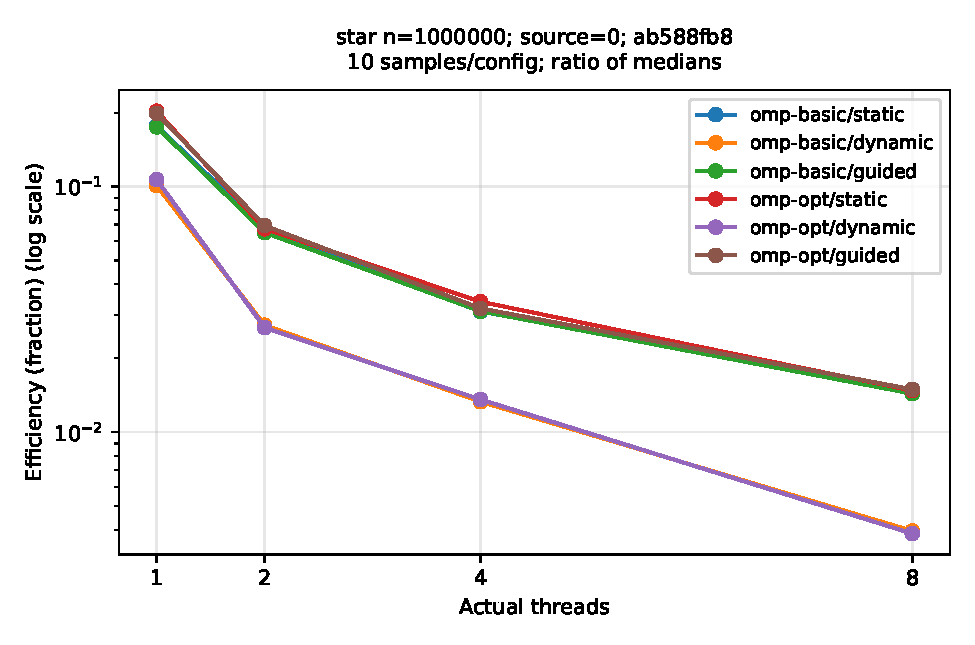
\includegraphics[width=.94\textwidth]{figures/experiment-20261112/star1000000-s0/efficiency.pdf}
\caption[Star1000000: efficiency]{Star1000000, nguồn 0: efficiency theo team thực, đơn vị phần số, không phải phần trăm.}\label{fig:star-efficiency}\end{figure}
\begin{figure}[p]\centering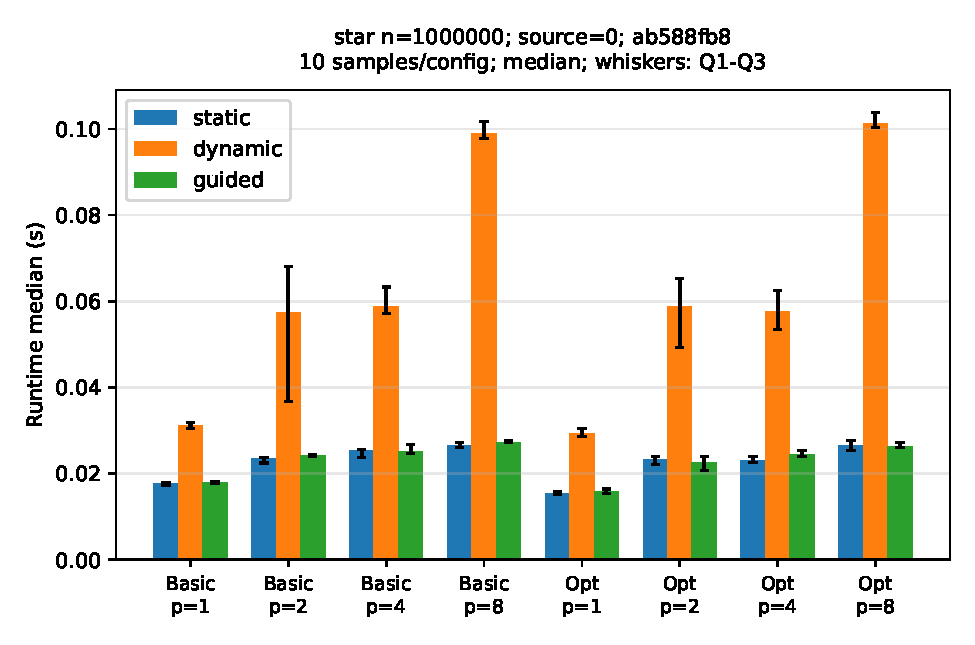
\includegraphics[width=.94\textwidth]{figures/experiment-20261112/star1000000-s0/scheduling.pdf}
\caption[Star1000000: scheduling]{Star1000000, nguồn 0: median và $Q_1$--$Q_3$ của ba schedule tại cùng team; dynamic chậm rõ ở nhiều luồng.}\label{fig:star-schedule}\end{figure}
\clearpage

\section{Grid: kích thước, số mức và nguồn}
Grid512 nguồn góc có Serial median 1,6942 ms, Basic8/static 112,6744 ms và Optimized 179,7294 ms. Speedup là 0,01504 và 0,009426; efficiency0,188\% và 0,118\%. Từ grid128 lên grid512, số đỉnh gấp16 và số mức từ góc gần gấp4; Basic8/static tăng30,5277 lên 112,6744 ms (3,69 lần), Serial tăng18,6 lần. Xu hướng phù hợp ảnh hưởng mạnh của số mức, nhưng chưa tách mọi nguyên nhân từ timer tổng.

Nguồn tâm131328 giảm khoảng cách lớn nhất từ 1022 xuống512. Basic8/static còn 62,3913 ms (giảm 44,6\%), Optimized 92,5461 ms (giảm 48,5\%). Serial lại tăng1,6942 lên 1,87115 ms, nên không có một xu hướng cho mọi thuật toán. Frontier rộng hơn và ít mức hơn có thể giải thích thay đổi OpenMP; thứ tự truy cập và điều kiện phiên chưa kiểm soát hoàn toàn.

Ở nguồn góc/actual 8, dynamic cho Basic143,5954 ms và Optimized 224,1793 ms, lớn hơn static 27,4\% và 24,7\%. Guided nằm giữa:127,8383 và 190,7862 ms. Optimized một luồng/static thấp hơn Basic (5,814 so 7,0432 ms), nhưng 8 luồng lại cao hơn 59,5\%. Giảm contention có thể đổi lấy prefix/copy/barrier; dữ liệu không ủng hộ lợi ích ổn định qua team. Xem Hình~\ref{fig:grid-runtime}--\ref{fig:grid-schedule}.

\begin{figure}[p]\centering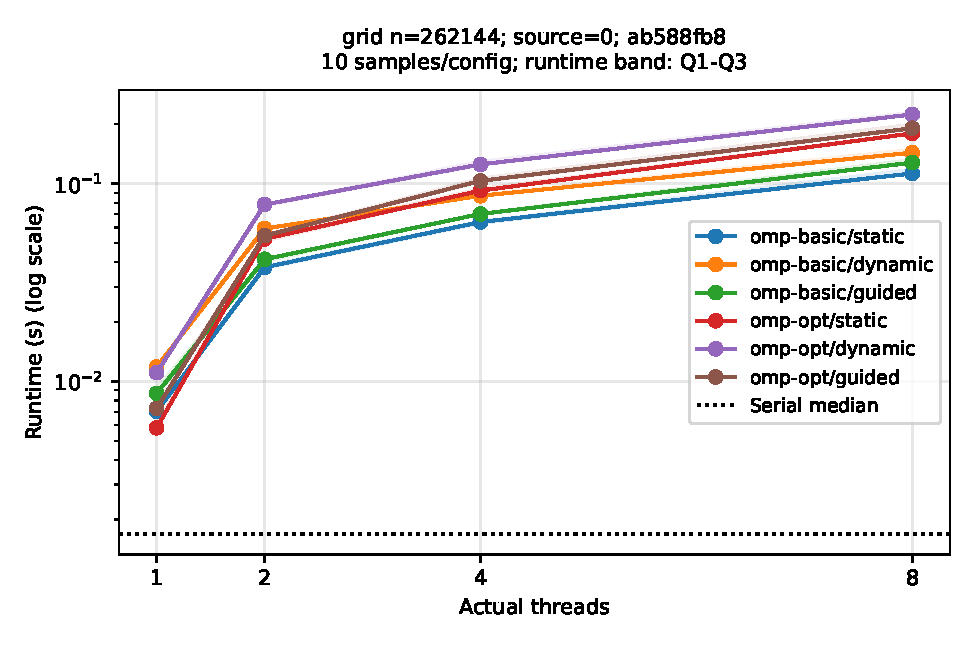
\includegraphics[width=.94\textwidth]{figures/experiment-20261112/grid512-s0/median.pdf}
\caption[Grid512: thời gian]{Grid512, nguồn 0: median và dải IQR thời gian; 10 mẫu/cấu hình, commit ab588fb.}\label{fig:grid-runtime}\end{figure}
\begin{figure}[p]\centering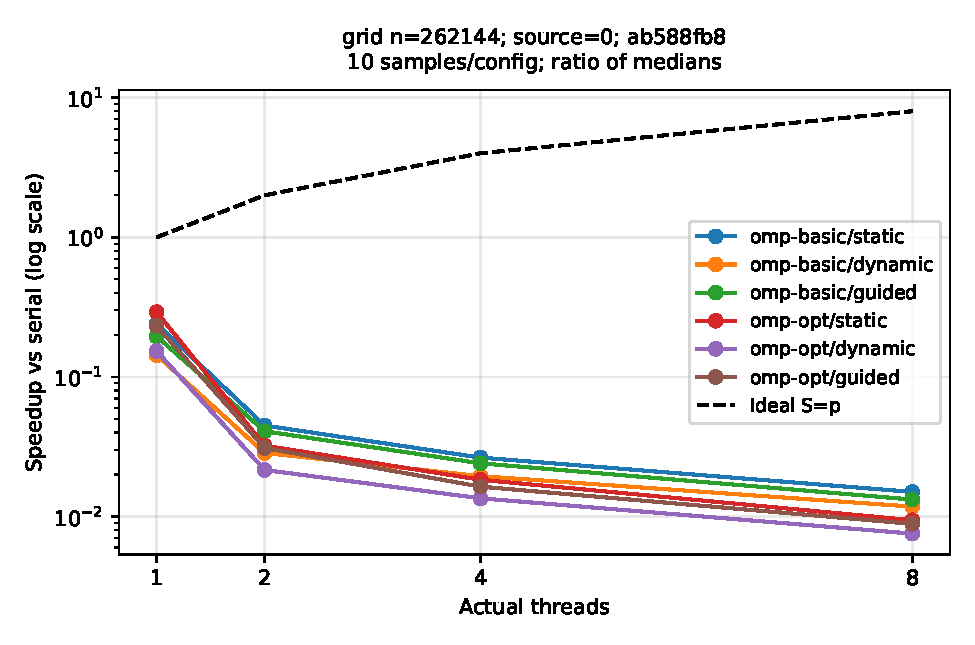
\includegraphics[width=.94\textwidth]{figures/experiment-20261112/grid512-s0/speedup.pdf}
\caption[Grid512: speedup]{Grid512, nguồn 0: speedup và mốc lý tưởng trên trục log. Optimized một luồng tốt nhất ma trận nhưng vẫn dưới 1.}\label{fig:grid-speedup}\end{figure}
\begin{figure}[p]\centering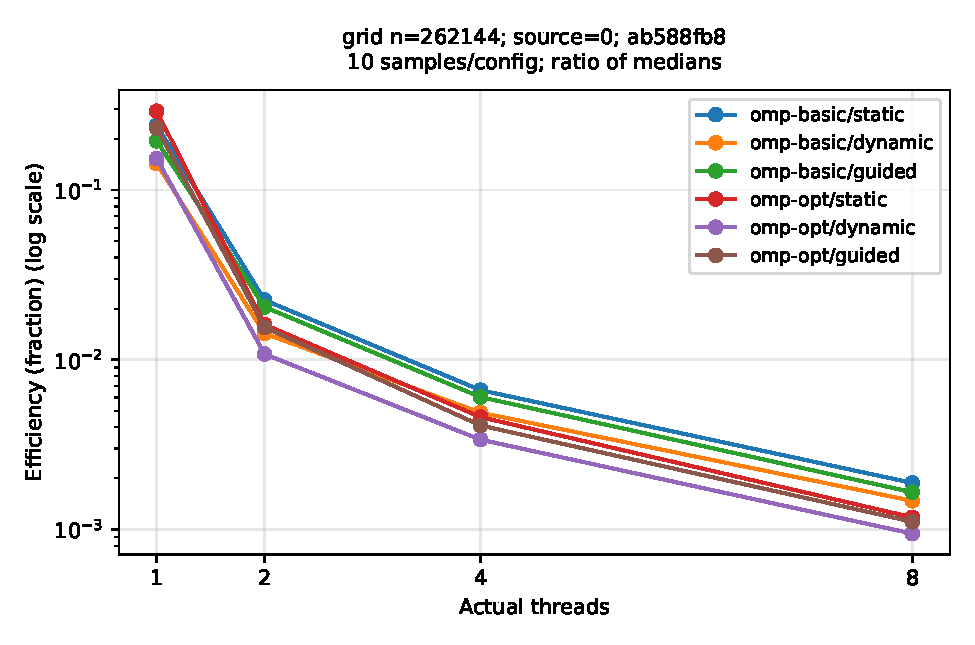
\includegraphics[width=.94\textwidth]{figures/experiment-20261112/grid512-s0/efficiency.pdf}
\caption[Grid512: efficiency]{Grid512, nguồn 0: efficiency theo actual team; không lấy requested threads thay team thực.}\label{fig:grid-efficiency}\end{figure}
\begin{figure}[p]\centering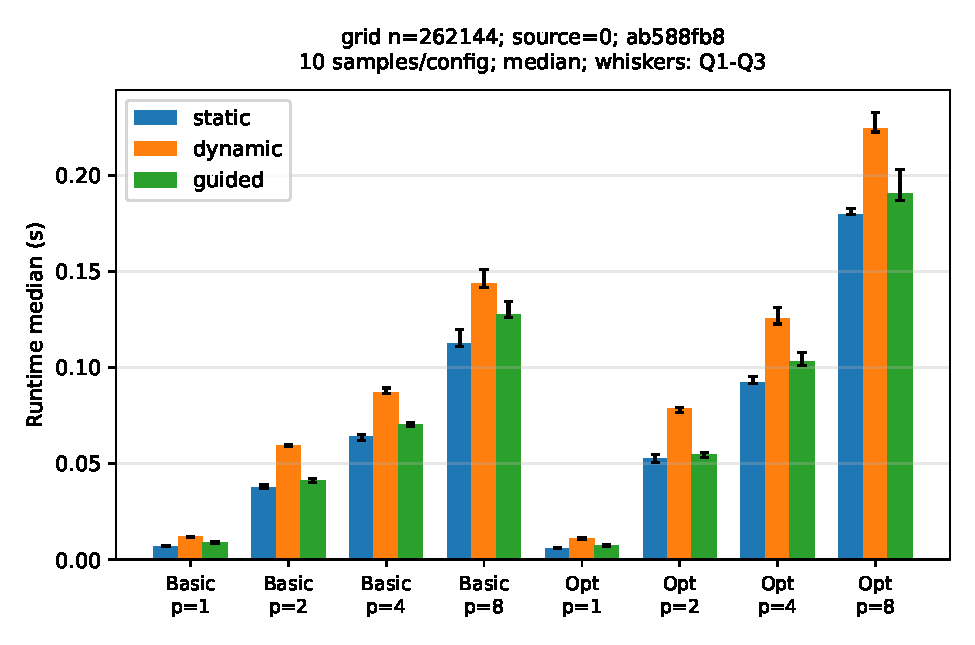
\includegraphics[width=.94\textwidth]{figures/experiment-20261112/grid512-s0/scheduling.pdf}
\caption[Grid512: scheduling]{Grid512, nguồn 0: median và $Q_1$--$Q_3$ của schedule tại cùng thuật toán/team.}\label{fig:grid-schedule}\end{figure}
\clearpage

\section{Đối chiếu câu hỏi nghiên cứu và độ tin cậy}
Correctness có oracle độc lập, full distance/CSR equality trong test và validation của 2475 lượt chạy; không quan sát lỗi trong phạm vi đã thử. Khả năng mở rộng không cho thấy tăng tốc: cả 216 cấu hình OpenMP có $S<1$, mọi cấu hình từ hai luồng có $C<1$. Hiệu năng thấp không làm kết quả khoảng cách trở thành sai, nhưng bác bỏ kỳ vọng tăng tốc cho phép đo này.

Optimized/scheduling phụ thuộc cấu hình: Optimized có median tốt hơn Basic ở một số cấu hình một/bốn luồng, song chậm hơn rõ trên path/grid ở 8 luồng; dynamic thường thêm chi phí trên star/grid. Không có bằng chứng một phiên bản/schedule luôn thắng. Các tỉ số mô tả median, chưa phải kiểm định thống kê khác biệt trung bình.

IQR/median lớn nhất khoảng 67,0\% ở Serial/star100000: median 0,2825 ms, min0,1870, max0,6137, $Q_1=0,1926$, $Q_3=0,381825$ ms. Mọi mẫu vẫn được giữ. Chênh lệch nhỏ hơn mức phân tán cần diễn giải thận trọng; QPC chỉ giải quyết lượng tử hóa1 ms, không loại tải nền hoặc scheduling Windows.

Dataset/nguồn chạy theo từng khối; shuffle chỉ trong khối nên còn sai lệch giữa thời điểm. Một máy, đồ thị có cấu trúc, team mới mỗi process, không affinity/profiling/nhiệt độ hoặc máy thứ hai là các giới hạn chính. Chưa có cơ sở suy luận về frontier rộng bất quy tắc hoặc BFS lặp với team đã nóng. sessions.json liên kết bảng/đồ thị với session, commit và manifest/raw hashes; summary.csv giữ đầy đủ thống kê để kiểm tra lại.

\chapter{Kết luận và hướng phát triển}
\section{Đóng góp và câu trả lời nghiên cứu}
Nhóm đã tích hợp Serial, OpenMP Basic và Optimized qua cùng CSR bất biến, API v1 và validation ngoài timer; cài và kiểm tra thật GCC/libgomp UCRT64 trên laptop Windows. Bộ công cụ giữ raw, lỗi, thứ tự, warm-up, actual team, manifest và SHA-256; analyzer từ chối thiếu cấu hình, plotter tách speedup so Serial khỏi scaling so OpenMP một luồng. Quyết định QPC được ghi rõ sau khi phát hiện giới hạn timer OpenMP Windows.

Câu hỏi correctness được hỗ trợ bởi oracle độc lập,1296 integration BFS calls, tests A/B/C và 2475 lượt thực nghiệm không lỗi. Đây là bằng chứng hữu hạn và review đồng bộ, không phải chứng minh tuyệt đối không có race.

Với khả năng mở rộng,2250 mẫu trên chín tổ hợp đồ thị/nguồn không ghi nhận $S>1$. Speedup tốt nhất là 0,2914 ở Optimized một luồng/static/grid512 nguồn 0. Basic 8/static có speedup 0,00005623 trên path8192,0,1185 trên star một triệu đỉnh và 0,01504 trên grid512. Mọi cấu hình nhiều luồng chậm hơn OpenMP một luồng cùng schedule. Tập cấu hình và mô hình lời gọi độc lập này chưa khai thác đa nhân hiệu quả.

Optimized không thắng nhất quán. Trên grid512 nguồn 0/static, một luồng Optimized thấp hơn Basic (5,814 so 7,0432 ms), nhưng 8 luồng cao hơn (179,7294 so 112,6744 ms). Dynamic làm star một triệu đỉnh/8 luồng chậm hơn static khoảng 3,7--3,8 lần. Cần đánh giá đồng thời tổ chức frontier, công việc hữu ích và chi phí lập lịch/đồng bộ, thay vì suy từ số lõi hoặc tên phiên bản.

\section{Giới hạn và bài học}
Kết luận chỉ áp dụng cho laptop/build/dataset đã mô tả, một BFS trong mỗi tiến trình mới. Warm-up không tạo team đã nóng cho mẫu sau; khởi tạo team trong BFS được tính. Mười mẫu và IQR không thay khoảng tin cậy hoặc tái lập độc lập. Không đo nhiệt độ, affinity theo loại lõi, cache miss, băng thông hay từng barrier; nguồn/kích thước chạy theo khối nên còn ảnh hưởng thời điểm. Không lấy timing CI hoặc bỏ outlier để làm kết quả đẹp hơn.

Path có frontier hẹp; star có một đỉnh bậc cao nhưng vòng láng giềng chưa song song; grid có nhiều mức tương đối hẹp. Chúng là phép thử có ý nghĩa nhưng chưa bao phủ frontier rất rộng bất quy tắc. OpenMP chậm ở đây không bác bỏ khả năng tăng tốc trên cấu trúc, runtime hoặc triển khai khác.

\section{Hướng phát triển}
Ưu tiên profiling để định lượng đồng bộ, visited và ghép frontier trước khi sửa thuật toán. Có thể thiết kế protocol riêng cho nhiều BFS cùng tiến trình/team đã nóng, đồng thời giữ phép đo lời gọi độc lập; không gộp hai mô hình thành một baseline. Chia công việc theo cạnh hoặc khảo sát direction-optimizing~\cite{beamer2012} là hướng khác, chưa phải phần đã triển khai.

Thực nghiệm tiếp theo nên đăng ký trước đồ thị layered/ngẫu nhiên seed cố định, nguồn và kích thước frontier rộng, kiểm soát thứ tự giữa các khối rồi tái lập trên máy khác. Mọi thay đổi vẫn cần oracle và provenance. Báo cáo/bảng/biểu đồ/raw được chuẩn bị để nghiệm thu độc lập; CI và review hỗ trợ AI không thay approval của thành viên có quyền.

\paragraph{Ghi nhận cách tổ chức báo cáo.} Tham khảo cấu trúc trình bày của mẫu SVD~\cite{svdtemplate}, không sử dụng nội dung chuyên môn hoặc số liệu của mẫu.

\nocite{trobec2018,parallelbfs,svdtemplate}
\bibliographystyle{plain}
\phantomsection
\addcontentsline{toc}{chapter}{Tài liệu tham khảo}
\bibliography{references}
\end{document}
